\documentclass[a4paper,11pt]{article}

\usepackage{../general/preamble}
\usepackage[onehalfspacing]{setspace}

\begin{document}

\begin{titlepage}
    \begin{center}
        \vspace*{1cm}
 
        \Large{\textbf{Homotopietypen anhand kritischer Werte}}
 
        \vspace{0.5cm}
        Ein Vortrag für das Seminar \\ 
        "Topics in Global Analysis" \\
        bei Frau Ursula Ludwig
             
        \vspace{1.5cm}
 
        \textbf{Jakob Dimigen}
             
    \end{center}
\end{titlepage}

\section{Einführung}

Sei $M$ eine glatte Abbildung, $f: M \to \R$ eine glatte Abbildung, 
$a \in \R$. Dann ist $M^a = f^{-1}(- \infty, a]$ ein \textit{sublevel set} von 
$f$. Das Ziel des Vortrags ist es, die Topologie der sublevel sets einer 
Abbildung mit ausschließlich nicht degenerierten kritischen Punkten, so genannten
\textit{Morsefunktionen}, zu verstehen.
Wir Untersuchen die Situation anhand des Torus. Wir stellen uns Morsefuinktionen
der einfachheitshalber als "Höhenfunktionen" vor.

\textbf{ZEICHNUNG Torus auf Ebene}

Es sei $f$ die Abbildung vom Torus nach $\R$, die jedem Punkt den minimalen
Abstand zu der eingezeichneten Ebene zuordnet. 
Die kritischen Punkte dieser Höhenfunktion sind $p$, $q$, $r$ und $s$.
Man stellt sich vor, dass man den Torus nach und nach mit Wasser befüllt. Dann 
ist für $a \in \R$ $M^a = f^{-1}(-\infty, a]$ die Menge der Punkte die bei der
Wasserhöhe $a$ das Wasser berühren. 

\begin{itemize}
    \item Für $a < 0$ ist $M^a = \varnothing$.
    \item Für $0 \leq a < f(p)$ ist $M^a$ homotopieäquivalent zum Punkt.
    \item Für $f(p) \leq a < f(q)$ ist $M^a$ homotopieäquivalent zum Kreis,
        an dem ein "Henkel" befestigt wurde.
    \item Für $f(q) \leq a < f(r)$ ist $M^a$ Homotopieäquivalent zum Zyliner,
        an dem ein "Henkel" befestigt wurde.
    \item Für $f(s) \leq$ ist $M^a$ der Torus selbst.
\end{itemize}

Wir bemerken: 
\begin{itemize}
    \item Gibt es im Intervall $[a, b]$ keine kritischen Werte, so haben alle
        $M^c$ für $c \in [a, b]$ denselben Homotopie-Typ
    \item Gibt es im Intervall $[a, b]$ genau einen kritischen Wert $c$ und ist
        $ \#f^{-1}(p) = 1$, dann hat $M^b$ den Homotopie-Typ von $M^a$ mit einem 
        Henkel angebracht (Was auch immer das bedeutet).
\end{itemize}

Um diese zwei Aussagen zu präzisieren, brauchen wir einige Definitionen:

\begin{definition}[Deformationsretrakt]
    Sei $X$ ein topologischer Raum und $A \subseteq X$ ein Unterraum von $X$.
    Eine stetige Abbildung $r: X \times [0, 1] \rightarrow X$ heißt 
    \textit{Deformationsretraktion} auf $A$, falls gelten:
    \begin{align*}
        & r(\cdot, 0) = \id_X \\
        & r(X, 1) \subseteq A \\
        & r(\cdot, 1)|_A = \id_A \\
    \end{align*}
    $A$ heißt \textit{Deformationsretrakt}, falls eine Deformationsretraktion
    von $X$ auf $A$ existiert.
\end{definition}

Deformationsretrakte haben einige schöne Eigenschaften. Falls $A$ ein
Deformationsretrakt von $X$ ist, so ist die Inklusion $A \rightarrow X$ eine
Homotopieäquivalenz. Da Homotopieäquivalenz transitiv ist, hat ein weiterer
Deformationsretrakt $B$ von $X$ deshalb denselben Homotopietypen wie $A$. \\
Es eine Tatsache, dass zwei Unterräume $A$ und $B$ genau dan denselben 
Homotopietypen haben, wenn sie beide Deformationsretrakte eines gemeinsamen 
Oberraumes sind. Um dies einzusehen benötigt man weitere topologische 
Theorie.

\begin{definition}[Eine $k$-Zelle anbringen]
    Es sei $X$ ein Topologischer Raum. Seien
    \[ e^k = D^k = \{(x_1, ..., x_k) \in \R^k: x_1^2 + ... + x_k^2 \leq 1\} \]
    \[ \varphi: \del e^k \rightarrow X \text{ stetig } \]
    \[ X \cup_{\varphi} e^k = (X \amalg e^k) / \sim, \text{ wobei } \]
    \[ \del e^k \ni x \sim y \in X \Leftrightarrow \varphi(x) = y \]
    Dann heißt $e^k$ $\lambda$-Zelle, $\varphi$ Anheftungsabbildung 
    und $X \cup_{\varphi} e^k$ heißt $X$ mit einer $k$-Zelle 
    angebracht.
\end{definition}

\textbf{ZEICHNUNG 1-Zelle, 2-Zelle}

Ein Paar Beispiele: 
\begin{itemize}
    \item Eine $0$-Zelle in einen nichtleeren Raum anzubringen 
        verändert diesen nicht, und
        \[\varnothing \cup_{\varphi} e^0 = \ast\]
    \item Eine $1$-Zelle lässt uns Zusammenhangskomponenten mit einer "Schnur"
            verbinden, oder ist das Anheften einer "Schlaufe".
    \item Eine $2$-Zelle anzubringen kann sein wie das anbringen einer Blase oder
        das stopfen eines Loches durch eine "Membran".
\end{itemize}

Eine $k$-Zelle kann also zwei Sachen: "Löcher", die von der $k$-ten Homologie
"gemessen" werden zu erschaffen oder "Löcher", die von der $(k-1)$-ten Homologie
"gemessen" werden zu "stopfen". Wenn wir also unsere Mannigfaltigkeit in 
Bezug auf solche Zellen bringen können, dann macht es uns das leichter die 
Topologie (und Homologie) der Mannigfaltigkeit besser zu verstehen. Wenn wir
sogar die gesamte Mannigfaltigkeit durch iteratives anbringen von $k$-Zellen
an den leeren Raum "erschaffen" können, dann können wir einigen Aussagen über 
die Homologie des Raumes machen. 


\begin{theorem}[Erstes Deformationslemma]
    \label{theorem:erstes deformationslemma}
    Es sei $M$ eine glatte Mannigfaltigkeit und $f: M \rightarrow \R$ eine
    glatte Abbildung. Hat $f$ keine kritischen Werte im Intervall [a, b] und ist
    $f^{-1}[a, b]$ kompakt, so existiert ein Diffeomorphismus 
    $M^a \rightarrow M^b$, und $M^a$ ist ein Deformationsretrakt von $M^b$.
\end{theorem}

\begin{theorem}[Zweites Deformations-Lemma]
    \label{theorem:zweites deformations-lemma}
    Es sei $M$ eine glatte Mannigfaltigkeit, $f: M \rightarrow \R$ eine glatte
    Abbildung und $p$ ein nicht-degenerierter kritischer Punkt mit Index 
    $\lambda$. Sei $c := f(p)$ und $\varepsilon \geq 0$, sd. 
    $f^{-1}[c - \varepsilon, c + \varepsilon]$ kompakt ist und außer $p$ keine 
    weiteren kritischen Punkte von $f$ beinhaltet. Dann hat $M^{c-\varepsilon}$
    denselben Homotopietypen wie $M^{c - \varepsilon} \cup_{\varphi} e^{\lambda}$
    für eine Anheftungsabbildung 
    $\varphi: \del e^{\lambda} \rightarrow M^{c-\varepsilon}$
\end{theorem}

\section{Das erste Deformationslemma}

Die Idee des Beweises ist es, $M^a$ entlang der Richtung, in die $f$ am stärksten
steigt, also parallel zum "Boden" via eines Diffeomorphismus $\varphi$ "nach oben 
zu ziehen", bis $\varphi(f^{-1}(a)) = f^{-1}(b)$. Dazu benötigen wir ein paar 
Werkzeuge:

\begin{definition}[Riemannsche Metrik]
    Bemerke: $( TM \otimes TM )^*$ ist Isomorph zu dem Vektorbündel mit Fasern 
    $\operatorname{Bil}(T_pM, \R)$. Eine \textit{Riemannsche Metrik} ist eine glatte
    Section $g: M \to (T^M \otimes T^M)^*$; $g(p) = g_p = \langle \cdot, \cdot \rangle$, 
    sodass $g_p$ für alle $p \in M$ ein Skalarprodukt ist.
\end{definition}

\begin{definition}[Gradient]
    Es sei $M$ \textit{Riemannsche Mannigfaltigkeit}, also eine Mannigfaltigkeit
    zusammen mit einer Riemannschen Metrik $g$. Außerdem sei $f: M \to \R$ glatt.
    Dann ist der \textit{Gradient} von $f$ $\grad f$ das (einzigartige) 
    Vektorfeld, für das gilt:
    \[ \langle X, \grad f \rangle = \opd fX \]

    \textbf{ZEICHNUNG: gradient einer Höhenfunktion}
\end{definition}

\begin{definition}[Flusslinie, Wang]
    Es sei $X$ ein Vektorfeld auf einer glatten Mannigfaltigkeit $M$. Für einen
    glatten Weg $\gamma: I \to M$, $I \subseteq \R$ ein Intervall, 
    definieren wir
    \[ \dot{\gamma}(t) \in T_pM \text{ für } p = \gamma(t) \text{ für ein } t \in I \text{ durch } 
    \dot{\gamma}(t) = \opd \gamma (t) \left(\derive{t}\right) \]
    wobei $\derive{t} \in T_pM$ das durch die Standardbasis von $\R$
    induzierte Element im Tangentialraum ist.
    Ein Weg $\gamma: I \to \R$ heißt \textit{Flusslinie} eines Vektorfeldes $X$,
    falls für alle $t \in I$ gilt:
    \[ X(\gamma(t)) = \dot{\gamma}(t) \]
\end{definition}

\begin{definition}[1-Parameter Gruppe aus Diffeomorphismen]
    Eine \textit{1-Parameter Gruppe aus Diffeomorphismen} ist eine glatte 
    Abbildung
    \[ \varphi: \R \times M \to M \text{, wobei } (t, p) \mapsto \varphi_t(p) = \varphi^p(t) \]
    Sodass für alle $s$, $t \in \R$ gilt:
    \[ \varphi_{t + s} = \varphi_t \circ \varphi_s \]
    und 
    \[ \varphi_0 = \id_M \]
    Wir sagen eine 1-Parameter Gruppe aus Diffeomorphismen wird von einem
    Vektorfeld $X$ generiert, falls für alle $p \in M$ gilt
    \[ X(p) = \dot{\varphi^p}(0) \]
\end{definition}

Ist $\varphi$ eine 1-Parameter Gruppe aus Diffeomorphismern, so ist für alle 
$t \in \R$ $\varphi_t$ ein Diffeomorphismus mit Inverse $\varphi_{-t}$.

Bemerke: Falls $X$ eine 1-Parameter Gruppe aus Diffeomorphismen $\varphi$ erzeugt,
dann ist für alle $p \in M$ der Weg $\varphi^p$ eine Flusslinien von $X$, denn
\begin{align*}
    X(\varphi^p(t)) 
    & = \dot{\varphi^{\varphi^p(t)}}(0)
    = T_0 \varphi^{\varphi^p(t)} \left(\derive{t}\right) \\
    & = T_0 \varphi_{t + \id_{\R}}(p) \left(\derive{t}\right)
    = T_t \varphi_{\id_{\R}}(p) \cdot T_0 (t + \id_{\R}) \left(\derive{t}\right) \\
    & = T_t \varphi_{\id_{\R}}(p) \left(\derive{t}\right)
    = T_t \varphi^p \left(\derive{t}\right) \\
    & = \dot{\varphi^p}(t)
\end{align*}

\begin{lemma}
    \label{lemma:generierende vektorfelder}
    Es sei $X$ ein Vektorfeld auf einer glatten Mannigfaltigkeit $M$, sodass
    $\supp(X)$ kompakt. Dann generiert $X$ eine eindeutige 
    1-Parameter Gruppe aus Diffeomorphismen.
\end{lemma}

\begin{proof} Der Beweis wird ausgelassen. \end{proof}

\begin{proof}[Erstes Deformations-Lemma]
    Es existiert eine kompakte Umgebung $K \in M$ von $f^{-1}[a, b]$. Dies folgt
    aus Whitneys Einbettungssatz und dem Satz von Heine-Borel.
    Sei $\rho: M \to \R$ eine glatte, positive Funktion, sodass
    \[ \rho(p) = 1 / \langle \grad f, \grad f \rangle \]
    für alle $p \in f^{-1}[a, b]$ und die außerhalb von $K$ verschwindet und für
    die für $p \in K$, die keine kritischen Punkte sind, gilt: 
    \[ 0 \leq \rho(p) \leq 1 / \langle \grad f, \grad f \rangle \]
    Bemerke dass $\rho$ innerhalb von $f^{-1}[a, b]$ wohldefiniert 
    ist, da sich keine kritischen Punkte im Intervall $[a, b]$ befinden. 
    Definiere ein Vektorfeld $X$ durch
    \[ X(p) = \rho(p) \cdot \grad f (p) \]
    Dann hat $X$ kompakten Träger, erfüllt also die Vorraussetzungen von 
    Lemma~\ref{lemma:generierende vektorfelder}. Sei also $\varphi$ die
    einzigartige 1-Parameter Gruppe aus Diffeomorphismen, die von $X$ generiert
    wird. 
    Wir bekommen für jedes $p \in M$ eine Abbildung $f \circ \varphi^p: \R \to \R$.
    
    \proofheading{Behauptung 1} Für alle $p \in M$, $t_0 \in \R$ und $q = \varphi^p(t_0)$
    ist $\derive{t} f \circ \varphi^p (t_0) \in [0, 1]$ und falls $f(\varphi^p(t)) \in [a, b]$
    gilt sogar $\derive{t} f \circ \varphi^p (t_0) = 1$.

    Für $q = \varphi_{t_0}(p)$:
    \begin{align*}
        \derive{t} f \circ \varphi^p (t_0)
        & = T_{\varphi^p(t_0)} f \cdot T_{t_0}\varphi^p \left( \derive{t} \right)
        = \opd f (q) \cdot X(q) \\
        & = \langle X(q), \grad f (q) \rangle 
        = \rho(q) \langle \grad f (q), \grad f (q) \rangle \in [0, 1]
    \end{align*}
    
    $f \circ \varphi^p$ ist also monoton wachsend für alle $p \in M$, und in 
    $\supp (X)$ sogar streng monoton.

    Falls sogar $f(\varphi_p(t_0)) \in [a, b]$, dann gilt
    \[ \frac{d}{dt} f \circ \varphi^p (t_0) = 1 \]
    \sectiondone

    \proofheading{Behauptung 2} Für $p \in f^{-1}(a)$, $t_0 \in [0, b-a]$ gilt $f(\varphi_p(t_0)) \in [a, b]$.
    
    \[ f(\varphi_{t_0}(p)) \geq f(\varphi_0(p)) = a \]
    und
    \begin{align*}
        f(\varphi_t(p)) 
        & \leq f(\varphi_{b-a}(p)) \\
        & = \int_0^{b-a}\derive{t} f(\varphi_t(p)) \opd t + f(\varphi_0(p)) \\
        & = \int_0^{b-a}\rho(\varphi_t(p)) \langle \grad f (\varphi_t(p)), \grad f (\varphi_t(p)) \rangle \opd t + a \\
        & \leq \int_0^{b-a} 1 \, \opd t + a \\
        & = b
    \end{align*}
    \sectiondone

    \textbf{ZEICHNUNG: In $f^{-1}[a, b]$ ist $f \circ \varphi^p$ linear mit Steigung $1$}

    \proofheading{Behauptung 3} Unter $\varphi_{b-a}$ wird das Level-Set 
    $f^{-1}(a)$ auf das Level-Set $f^{-1}(b)$ abgebildet.
     
    Für $p \in f^{-1}(a)$ gilt:
    \[ \varphi_{a-a}(p) = \varphi_0(p) = p \]
    und für $t_0 \in [0, b - a]$ gilt wegen Behauptung 2
    \[ \derive{t}f(\varphi^p(t-a)) (t_0) = 1 \]
    also
    \[ f(\varphi^p(b-a)) = f(\varphi_{0}(p)) + (b - a) = b \]
    Genauso gilt für $q \in f^{-1}(b)$: $f(\varphi_{a - b}(q)) = a$, also 
    $\varphi_{b - a}(f^{-1}(a)) = f^{-1}(b)$.
    \sectiondone

    \proofheading{Behauptung 4} Für $p, q \in M$ und $t \in \R$ gilt:
    \[ f(p) \leq f(q) \Leftrightarrow f(\varphi_t(p)) \leq f(\varphi_t(q)) \]

    Seien oBdA $p, q \in \supp (X)$.

    "$\Rightarrow$": $f \circ \varphi^p: {\varphi^p}^{-1}(\supp(X)) \to f(\supp(X))$
    ist monoton und surjektiv. Wegen der Surjektivität von $f \circ \varphi^q $ 
    existieren $q' \in \supp(X)$, $s > 0$ sodass
    \[ \varphi_{t + s}(p) = \varphi_t(q') \text{ und } f(\varphi_t(q')) = f(\varphi_t(q)) \]
    Wegen der Monotonie gilt dann
    \[ 
        f(\varphi_t(q)) = f(\varphi_t(q')) = f(\varphi_t(\varphi_s(p))) 
        = f(\varphi_{t+s}(p)) = f(\varphi^p(t+s)) \geq f(\varphi^p(t)) = 
        f(\varphi_t(p)) \]

    "$\Leftarrow$": Setze $\tilde{p} := \varphi_{-t}(p)$ und $\tilde{q} := \varphi_{-t}(q)$.
    Gilt 
    \[ 
        (f(p) \leq f(q) \Leftarrow f(\varphi_t(p)) \leq f(\varphi_t(q)))
        \Leftrightarrow 
        (f(\varphi_t(\tilde{p})) \leq f(\varphi_t(\tilde{q}))) \Leftarrow f(\varphi_t(\tilde{p})) \leq f(\varphi_t(\tilde{q}))
    \]
    Was schon gezeigt wurde.

    \sectiondone

    \proofheading{Behauptung 5} Es gilt $\varphi_{b-a}(M^a) = M^b$.
   
    "$\subseteq$": Sei $p$ in $M^a$, oBdA. $p \in \supp(X)$, ansonsten gilt
    \[ \varphi_{b-a}(p) = p \in M^b \]
    Sei $q \in f^{-1}(a)$. Dann gilt 
    \[ f(\varphi_{b-a}(p)) \leq f(\varphi_{b-a}(q)) = b \]
    "$\supseteq$": Analog
    \sectiondone

    Damit ist $\left. \varphi_{b-a} \right\vert_{M^a}$ ein Diffeomorphismus zwischen
    $M^a$ und $M^b$. 

    Betrachte nun $r: M^b \times \R \to M^b$,
    \[  
        r(p, t) = \begin{cases}
            p & \text{ falls } f(p) \leq a \\
            \varphi_{t(a - f(p))}(p) & \text{ falls } a \leq f(p) \leq b 
        \end{cases}
    \]

    Dann ist $r$ stetig, $r(\cdot, 0)$ ist die Identität auf $M^b$, 
    $r(\cdot, 1)|_{M^a}$ ist die Identität auf $M^a$ und 
    $r(1, M^b) \subseteq M^a$, also ist $M^a$ ein Deformationsretrakt von $M^b$.

\end{proof}

\section{Das zweite Deformationslemma}

Die Idee für den Beweis ist, sich eine neue Funktion $F: M \to \R$ zu definieren,
die Außerhalb von einer kleinen Umgebung von $p$ $f$ entspricht und in der 
Umgebung etwas kleiner ist. Dann bekommen wir die folgende Situation:

\textbf{ZEICHNUNG: Torus mit Delle}

Die Hoffnung ist dann, dass der Eingezeichnete "Henkel" Homotopieäquivalent zu
einer $\lambda$-Zelle ist.

\begin{proof}

    Sei $c := f(p)$. Mit dem Morse Lemma können wir lokale Koordinaten 
    $\varphi = u_1, ..., u_n)$ in einer Umgebung $U$ von $p$ wählen, sodass
    \[ f = c - u_1^2 - ... - u_k^2 + u_{k+1}^2 + ... + u_n^2 \]
    in dieser Umgebung. Dann gilt für den kritischen Punkt $p$:
    \[ u_1(p) = ... = u_n(p) = 0 \]

    Wähle nun $\varepsilon > 0$ klein genug, sodass 
    \begin{enumerate}
        \item $f^{-1}[c - \varepsilon, c + \varepsilon]$ kompakt ist und keine
            kritischen Punkte außer $p$ enthält
        \item $\{ x \in \R^n: \lVert x \rVert \leq 2 \varepsilon \} \subseteq \varphi(U) $
    \end{enumerate}

    Wähle nun die $k$-Zelle 
    \[ 
        e^k := \{ p \in M: (u_1(p))^2 + ... + (u_k(p))^2 \leq \varepsilon 
        \text{ und } u_{k+1}(p) = ... = u_n(p) = 0 \} 
    \]

    Wir bekommen die folgende Situation:

    \begin{figure}[H]
        \centering
        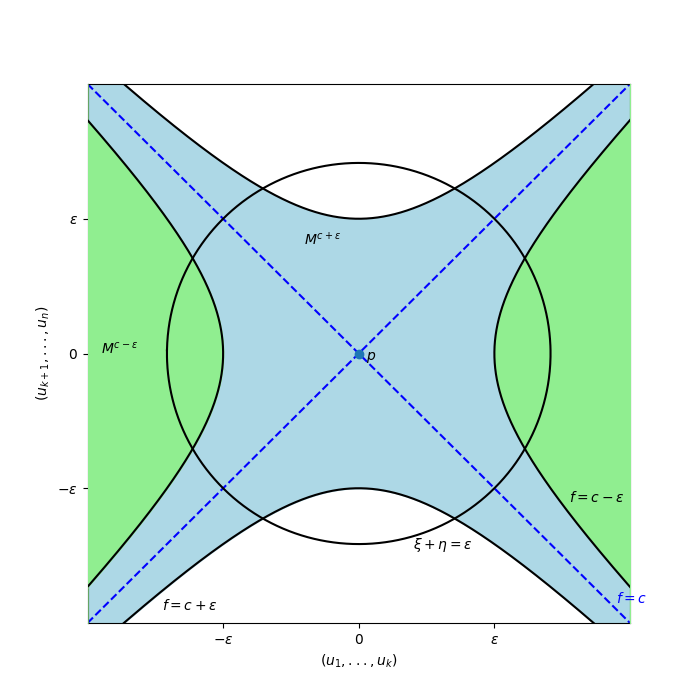
\includegraphics[width=0.8\linewidth]{resources/Me-Diagram6-parametrisierung-sattelpunkt.png}
        \label{fig:me-diagram6}
    \end{figure}

    Nun definiere eine glatte Funktion $\mu: \R \to \R$ mit den Eigenschaften:

    \begin{enumerate}
        \item $ \mu(0) > \varepsilon $
        \item $ \mu(r) = 0 $ falls $ r \geq 2 \varepsilon $
        \item $ -1 < \mu'(r) \leq 0 $ für alle $ r \in \R $
    \end{enumerate}

    Sei nun $F$ außerhalb von $U$ gleich $f$, und sei
    \[ F = f - \mu(u_1^2 + ... + u_k^2 + 2u_{k+1}^2 + ... + 2u_n^2) \]

    $F$ ist wohldefiniert und glatt, da $F$ außerhalb des Kreises mit Radius 
    $\sqrt{2\varepsilon}$ mit $f$ übereinstimmt und der gesamte Kreis in $U$ 
    enthalten ist.

    Wir definieren nun

    \begin{align*}
        & \eta, \xi: U \to [0, \infty) \\
        & \xi = u_1^2 + ... + u_k^2 \\
        & \eta = u_{k + 1}^2 + ... + e_n^2
    \end{align*}

    Dann gilt innerhalb von $U$:
    \[ f = c - \xi + \eta \]
    und 
    \[ F = f - \mu(\xi + 2 \eta) = c - \xi + \eta - \mu(\xi + 2 \eta) \]

    \proofheading{Behauptung 1} $F^{-1}(-\infty, c + \varepsilon] = M^{c + \varepsilon}$

    Sei $q \in M$. Falls gilt $\xi(q) + 2 \eta(q) > 2 \varepsilon$ gilt $f(p) = F(p)$,
    also gelte oBdA 
    \[ \xi(q) + 2 \eta(q) \leq 2 \varepsilon \]
    Dann:
    \[ F(q) \leq f(q) = c + \xi(q) + \eta(q) \leq c + \frac{1}{2}\xi(q) + \eta(q) \leq c + \varepsilon \]
    \sectiondone

    \proofheading{Behauptung 2} Die kritischen Punkte von $F$ stimmen mit denen 
    von $f$ überein.

    Bemerke, dass
    \[ \pderive[F]{\xi} = -1 - \mu'(\xi + 2\eta)  < 0 \]
    und
    \[ \pderive[F]{\eta} = 1 - 2 \mu'(\xi + 2\eta) \geq 1 \]
    Insbsondere sind diese beiden Ableitungen also niemals $0$. Da 
    \[ \opd F = \pderive[F]{\xi}\opd \xi + \pderive[F]{\eta} \opd \eta \]
    und $\opd \xi$ und $\opd \eta$ nur in $p$ Null sind, haben $f$ und $F$ 
    dieselben kritischen Punkte.
    \sectiondone

    \proofheading{Behauptung 3} $F^{-1}(-\infty, c - \varepsilon]$ ist ein
    Deformationsretrakt von $M^{c + \varepsilon}$.

    Betrachte die Region $F^{-1}[c - \varepsilon, c + \varepsilon]$. Wegen 
    Behauptung 1 und der Tatsache, dass $F \leq f$ gilt:
    \[ F^{-1}[c - \varepsilon, c + \varepsilon] \subseteq f^{-1}[c - \varepsilon, c + \varepsilon] \]
    Da $f^{-1}[c - \varepsilon, c + \varepsilon]$ kompakt ist und 
    $F^{-1}[c - \varepsilon, c + \varepsilon]$ abgeschlossen ist, ist 
    $F^{-1}[c - \varepsilon, c + \varepsilon]$ auch kompakt. Mit Behauptung 2
    kann diese Menge maximal den kritischen Punkt $p$ enthalten, aber
    \[ F(p) = c - \mu(0) < c - \varepsilon \]
    Also gibt es in $F^{-1}[c - \varepsilon, c + \varepsilon]$ keine kritischen
    Punkte. Mit dem ersten Deformationslemma und Behauptung 1 folgt die 
    Behauptung.
    \sectiondone

    Im Beweis von Behauptung 3 haben wir gesehen, dass 
    $M^{c - \varepsilon} \subseteq f^{-1}(-\infty, c - \varepsilon]$ und im
    Beweis von Behauptung 1, dass außerhalb des Kreises mit Radius 
    $\sqrt{2 \varepsilon}$ gilt $f = F$, also haben wir folgende Situation:
    
    \begin{figure}[H]
        \centering
        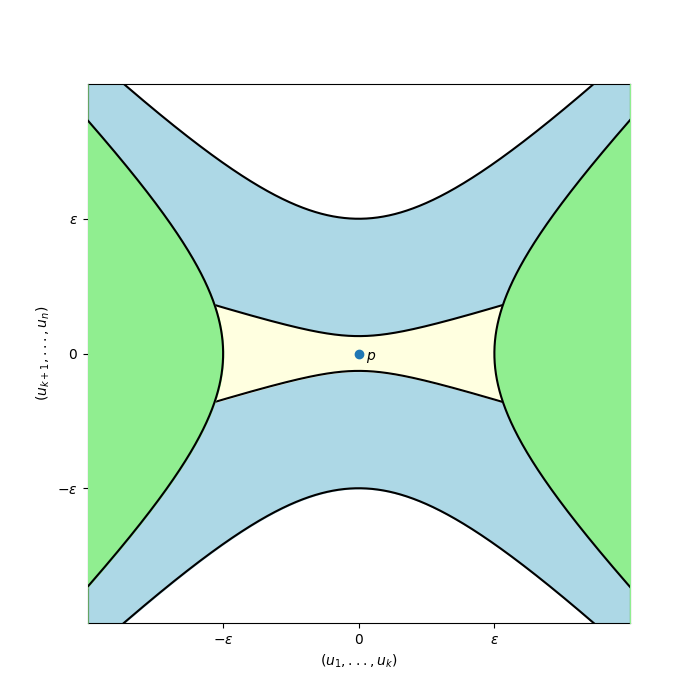
\includegraphics[width=0.8\linewidth]{resources/Me-Diagram7-handle.png}
        \label{fig:me-diagram7}
    \end{figure}

    Wir nennen nun $F^{-1}(-\infty, c-\varepsilon] - M^{c - \varepsilon} := H$.

    \proofheading{Behauptung 4} $M^{c - \varepsilon} \cup e^{k}$ ist ein 
    Deformationsretrakt von $M^{c - \varepsilon} \cup H$.

    Dafür konstruieren wir eine Deformationsretraktion
    $r: M^{c - \varepsilon} \cup H \times [0,1] \to M^{c - \varepsilon} \cup H$
    für $q \in M^{c - \varepsilon} \cup H, t \in [0, 1]$ wie folgt:
    \[
        r(q, t) = \begin{cases}
            \varphi^{-1} \circ (u_1, ..., u_k, tu_{k + 1}, ..., tu_n)(q)
                & \text{ im Fall 1: } \xi(q) \leq \varepsilon \\
            \varphi^{-1} \circ (u_1, ..., u_k, s_tu_{k + 1}, ..., s_tu_n)(q)
                & \text{ im Fall 2: } \varepsilon \leq \xi(q) \leq \eta(q) + \varepsilon \\
            q & \text{ im Fall 3: } \eta(q) + \varepsilon \leq \xi(q)
        \end{cases}
    \]

    Wobei 

    \[ s_t = t + (1 -t)((\xi - \varepsilon)/\eta)^{1/2} \]

    Die Fälle sind wie folgt:

    \begin{figure}[H]
        \centering
        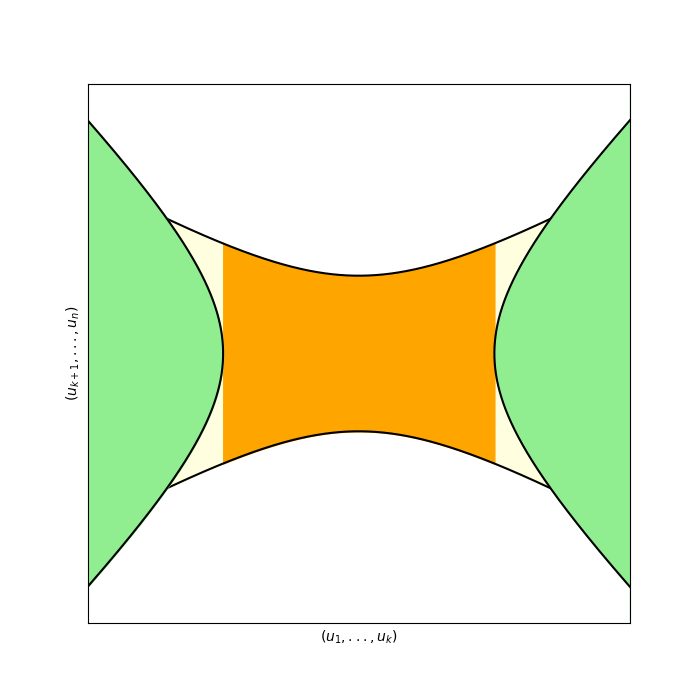
\includegraphics[width=0.8\linewidth]{resources/Me-Diagram9-handle-cases.png}
        \label{me-diagram9}
    \end{figure}

    Wir müssen überprüfen:
    \begin{enumerate}
        \item $r$ ist wohldefiniert und stetig
        \item $r(M^{c - \varepsilon} \cup H, 0) \subseteq M^{c - \varepsilon} \cup e^k$
        \item $r(\cdot, 1) = \id_{M^{c - \varepsilon} \cup H}$ und 
            $\left. r(\cdot , 0) \right\vert_{M^{c - \varepsilon} \cup e^k} 
            = \id_{M^{c - \varepsilon} \cup e^k}$
    \end{enumerate}

    3. ist einfach nachzurechnen. In Fall 1 und Fall 3 ist 2. offensichtlich
    wahr. Für Fall 2 gilt:
    \begin{align*} 
        f(r(0, q)) & = 
            f\left( \varphi^{-1} \left(u_1(q), ..., u_k(q), 
            \left( \frac{\xi(q) - \varepsilon}{\eta(q)} \right)^{1/2}u_{k + 1}(q), ...,
            \left( \frac{\xi(q) - \varepsilon}{\eta(q)} \right)^{1/2}u_n(q)
            \right)
            \right) \\
        & = c - \xi(q)
            + \left( \left( \frac{\xi(q) - \varepsilon}{\eta(q)} \right)^{1/2}u_{k + 1}(q) \right)^2 + ... 
            + \left( \left( \frac{\xi(q) - \varepsilon}{\eta(q)} \right)^{1/2}u_n(q) \right)^2 \\
        & = c - \left( \frac{\xi(q) - \varepsilon}{\eta(q)} \right) \eta(q) \\
        & = c - \varepsilon
    \end{align*}
    also ist $r(0, q) \in f^{-1}(c - \varepsilon)$. Um 1. zu prüfen müssen wir 
    Stetigkeit in den Grenzfällen überprüfen:
    \begin{align*}
        & \text{For } \xi(q) = \varepsilon \text{ : }
            & s_t(q)  =t + (1 - t)((\varepsilon - \varepsilon)/\eta(q))^{1/2} = t \\
        & \text{For } \eta(q) + \varepsilon = \xi(q) \text{ : }
            & s_t(q) = t + (1 - t)((\xi(q) - \varepsilon)/(\xi(q) - \varepsilon))^{1/2} = 1
    \end{align*}

    Das einzig andere Problem was wir bekommen könnten ist nun in Fall 2 falls
    $\eta \to 0$. In Fall 1 und Fall 3 bekommen wir für $q$ mit $\eta(q) = 0$:
    $r(q, t) = \varphi^{-1} \circ (u_1, ..., u_k, 0, ..., 0)(q)$, 

\end{proof}

\end{document}
